\documentclass[12pt] {article}

%%% Preambuła %%%
\usepackage[T1]{fontenc}
\usepackage[polish]{babel}
\usepackage[utf8]{inputenc}
\usepackage{lmodern}
\usepackage{hyperref}
\usepackage{mathptmx}
\usepackage{float}
\usepackage{graphicx}
\usepackage{xcolor}
\selectlanguage{polish}
\usepackage{titlesec}
\usepackage{listings}


\lstset{
	basicstyle=\ttfamily,
	columns=fullflexible,
	breaklines=true,
	breakatwhitespace=true,
	showstringspaces=false,
	commentstyle=\color{red},
	keywordstyle=\color{blue}
}

\definecolor{backgroundColor}{HTML}{3D3D3D}

%%% Strona tytułowa %%%
\title 
{	
	{
		\textbf{\textsf{\Huge\color{orange}DNS\color{white}ite}} \\ [0.1in]
		\normalfont\sffamily\LARGE\color{white}
		Aplikacja webowa do zarządzania serwerem DNS \\[0.1in]
		Dokumentacja użytkownika\\ [1.5in]
		\large 
		Inżynieria Oprogramowania \\
		Wydział Fizyki i Informatyki Stosowanej \\
		Informatyka Stosowana, 3 rok \\
	}
}

\author 
{
	\color{white}\normalfont\sffamily Arkadiusz Kasprzak \and 
	\color{white}\normalfont\sffamily Jarosław Cierpich \and 
	\color{white}\normalfont\sffamily Jakub Kowalski \and 
	\color{white}\normalfont\sffamily Konrad Pasik \and 
	\color{white}\normalfont\sffamily Krystian Molenda
}
\date{}


\definecolor{ao}{rgb}{0.0, 0.0, 1.0}	
\definecolor{forestgreen(web)}{rgb}{0.13, 0.55, 0.13}
\definecolor{darkbrown}{rgb}{0.4, 0.26, 0.13}
\definecolor{darkorange}{rgb}{0.91, 0.41, 0.17}

\titleformat{\section}
  {\normalfont\sffamily\Large\bfseries\color{darkorange}}
  {\thesection}{1em}{}

\titleformat{\subsection}
  {\normalfont\sffamily\large\bfseries\color{darkorange}}
  {\thesubsection}{1em}{}

\titleformat{\subsubsection}
  {\normalfont\sffamily\normalsize\bfseries\color{darkorange}}
  {\thesubsubsection}{1em}{}
	

\begin{document}


%%% Strona tytułowa %%%
\pagecolor{backgroundColor}
\maketitle
\thispagestyle{empty}


\newpage
\clearpage
\pagenumbering{arabic}
\pagecolor{white}

%%% Spis treści %%%
\tableofcontents

\newpage 

\section{Wstęp}
\textbf{DNSite} to aplikacja webowa do zarządzania serwerem DNS. Dostarcza ona użytkownikowi możliwości łatwej i wygodnej edycji danych związanych z serwerem PowerDNS przechowywanych w bazie PostgreSQL.\newline
Niniejsza dokumentacja użytkownika została przygotowana dla pierwszego pełnego wydania aplikacji. Zawiera instrukcję instalacji oraz konfiguracji aplikacji, jak również poradnik ułatwiający poznanie wszystkich funkcjonalności.

\section{Instalacja}
W celu uruchomienia aplikacji wymagane są:
\begin{itemize}
\item Java w wersji 8
\item Maven
\item Baza danych PostgreSQL 11
\item Aplikacja pgAdmin 4
\end{itemize}
Należy zadbać o to, by przed uruchomieniem aplikacji baza danych była już stworzona - może natomiast nie zawierać tabel.
W celu uruchomienia aplikacji należy pobrać ją z serwisu \textbf{Github} za pomocą polecenia:
\begin{lstlisting}[language=bash]
git clone https://github.com/agh-ki-io/DNSite
\end{lstlisting}
Następnie należy przejść do katalogu \emph{DNSite} za pomocą polecenia:
\begin{lstlisting}[language=bash]
cd DNSite
\end{lstlisting}
i wykonać z jego poziomu polecenie:
\begin{lstlisting}[language=bash]
mvn clean install
\end{lstlisting}
Proces instalacji może potrwać kilka minut. Należy zignorować pojawiające się komunikaty (również te oznaczone słowem \emph{error}). Po zakończeniu instalacji użytkownik powinien zobaczyć komunikat podobny do poniższego:
\begin{figure}[H]
\centering
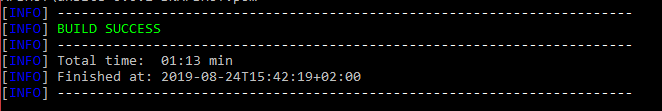
\includegraphics[width=\textwidth]{res/1_budowanie}
\end{figure}
Następnie w celu uruchomienia aplikacji należy \textbf{z poziomu katalogu DNSite} wykonać polecenie:
\begin{lstlisting}[language=bash]
java -jar target/dnsite-0.0.1-SNAPSHOT.jar
\end{lstlisting}
Krok ten należy wykonać za każdym razem, gdy aplikacja ma zostać uruchomiona. Należy teraz dokonać konfiguracji aplikacji (rozdział \hyperref[first_run]{\emph{Pierwsze uruchomienie i konfiguracja}}) lub, jeśli zostało to już zrobione, rozpocząć korzystanie z aplikacji za pomocą przeglądarki (rozdział \hyperref[webapp]{\emph{Korzystanie z aplikacji}}).

\section{Pierwsze uruchomienie i konfiguracja}
\label{first_run}
Rozdział omawia proces pierwszego uruchomienia aplikacji oraz sposoby na zmianę konfiguracji aplikacji.

\subsection{Pierwsze uruchomienie}
Podczas pierwszego uruchomienia aplikacji wyświetlone zostanie następujące okno:
\begin{figure}[H]
\centering
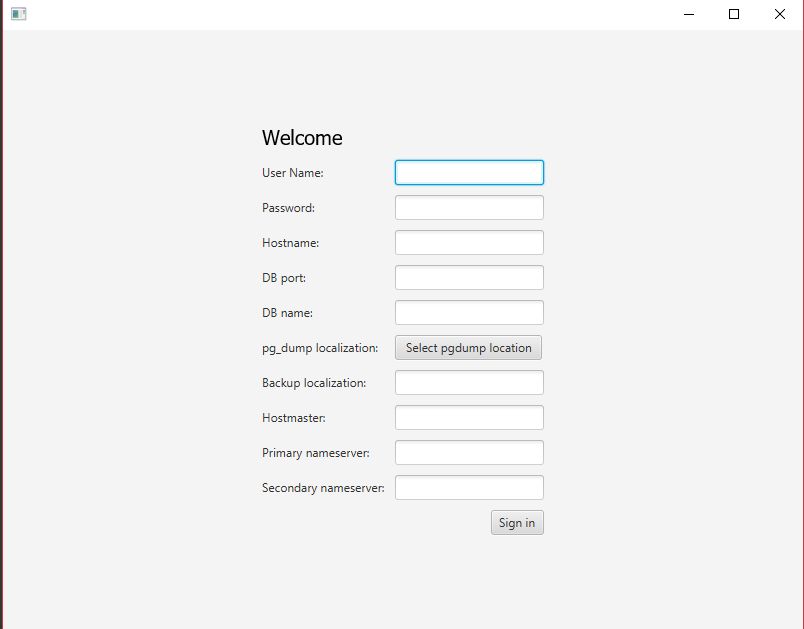
\includegraphics[scale=0.5]{res/2_konfiguracja}
\end{figure}
Służy ono do przeprowadzenia konfiguracji aplikacji - w szczególności wymaga od użytkownika szczegółów dotyczących bazy danych, z którą aplikacja ma się łączyć. Należy podać:
\begin{itemize}
\item Nazwę użytkownika posiadającego dostęp do bazy danych oraz prawa takie jak zapis czy odczyt z niej.
\item Hasło do bazy.
\item Nazwę hosta lub adres IP - np. \emph{localhost}.
\item Port, na którym dostępna jest baza.
\item Nazwę bazy danych, do której aplikacja ma się łączyć.
\end{itemize}
Ponadto interfejs zawiera dwa pola nieobowiązkowe:
\begin{itemize}
\item \emph{pg\_dump location} - ścieżka do narzędzie pg\_dump.exe, służącego do wykonywania kopii zapasowych danych z bazy PostgreSQL. Jest to oficjalne narzędzie dołączane przy instalacji programu pgAdmin.
\item \emph{Backup location} - ścieżka do katalogu, w którym przechowywane mają być kopie zapasowe danych z bazy
\end{itemize}
Ostatnie trzy pola są obowiązkowe:
\begin{itemize}
\item \emph{Hostmaster} - używane przy automatycznym tworzeniu rekordów SOA, gdy dodawana jest domena
\item \emph{Primary i Secondary nameserver} - domyślne serwery - podobnie jak wyżej, używane przy automatycznym tworzeniu rekordów SOA.
\end{itemize}
Po wprowadzeniu wszystkich koniecznych danych należy użyć przycisku \emph{Sign in}. Przeprowadzony zostanie test połączenia z bazą danych i jeśli zakończy się on pomyślnie, będzie można przejść do korzystania z właściwej części aplikacji.

\subsection{Zmiana konfiguracji}
Dostępne są dwa sposoby na ponowne przeprowadzenie procesu konfiguracji aplikacji:
\begin{itemize}
\item usunięcie pliku \textbf{dbconfig.yaml} - powoduje to ponowne uruchomienie opisanego powyżej graficznego interfejsu użytkownika przy następnym uruchomieniu aplikacji.
\item ręczna edycja pliku \textbf{dbconfig.yaml} - zapisane są w nim wszystkie parametry podane wcześniej za pomocą graficznego interfejsu użytkownika.
\end{itemize}
\newpage

\section{Korzystanie z aplikacji}
\label{webapp}
Dostęp do aplikacji można uzyskać \textbf{za pomocą przeglądarki}. Po uruchomieniu należy wpisać w pasku adresu \url{http://localhost:8001/}. \newline
Kolejne podrozdziały zawierają opis podstawowych operacji, jakie można wykonać w aplikacji, takich jak logowanie, rejestracja, zmiana hasła czy edycja danych przechowywanych w bazie (rekordy, domeny).

\subsection{Logowanie i rejestracja}
Po uruchomieniu aplikacji w przeglądarce użytkownik powinien uzyskać dostęp do strony umożliwiającej logowanie, zawierającej przedstawiony poniżej formularz:
\begin{figure}[H]
\centering
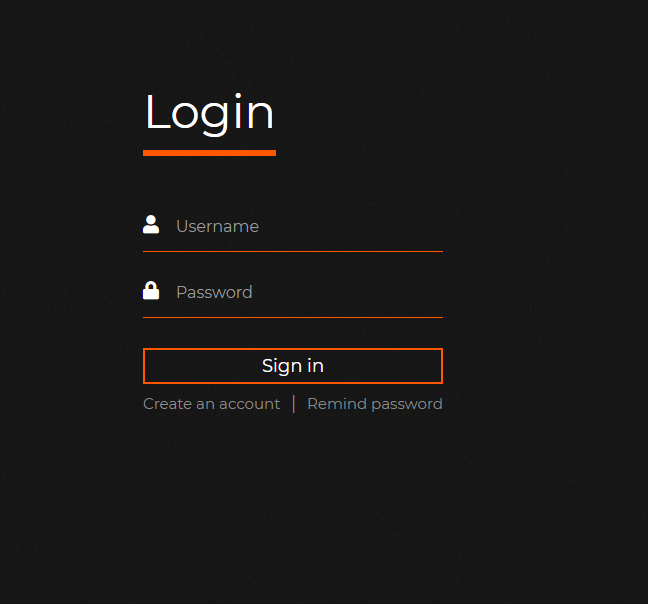
\includegraphics[scale=0.5]{res/3_logowanie}
\end{figure}
Umożliwia on wprowadzenie danych \textbf{logowania} (nazwa użytkownika i hasło ustalone przy rejestracji). W celu przeprowadzenie \textbf{rejestracji} należy wybrać opcję \emph{Create an account}. Wybranie jej przenosi do strony z następującym formularzem:
\begin{figure}[H]
\centering
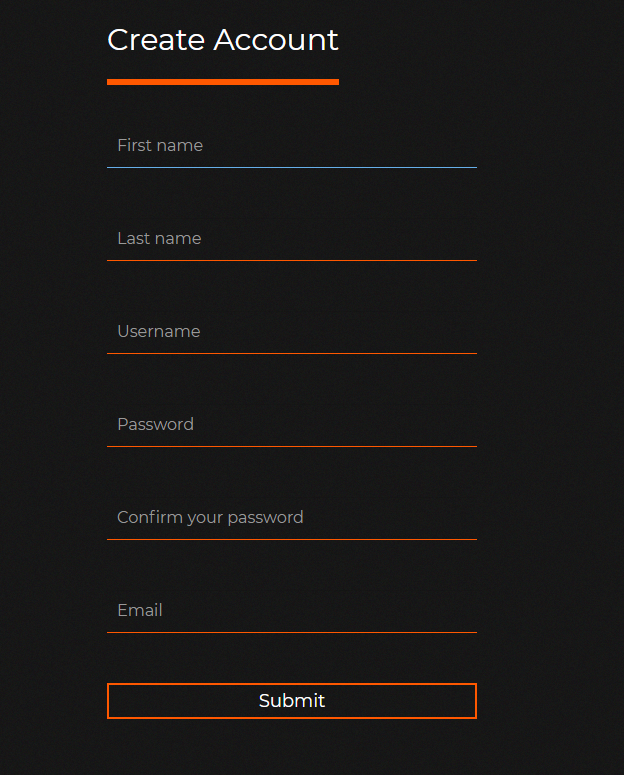
\includegraphics[scale=0.4]{res/4_rejestracja}
\end{figure}
Pierwszy utworzony użytkownik otrzymuje automatycznie prawa administratora i dostęp do aplikacji. Każdy następny musi zostać zatwierdzony przez zweryfikowane już konto (czyli konto mające dostęp do aplikacji). Do właścicieli takiego konta wysyłana jest wiadomość e-mail z powiadomieniem. Poniżej przykład takiej wiadomości:
\begin{figure}[H]
\centering
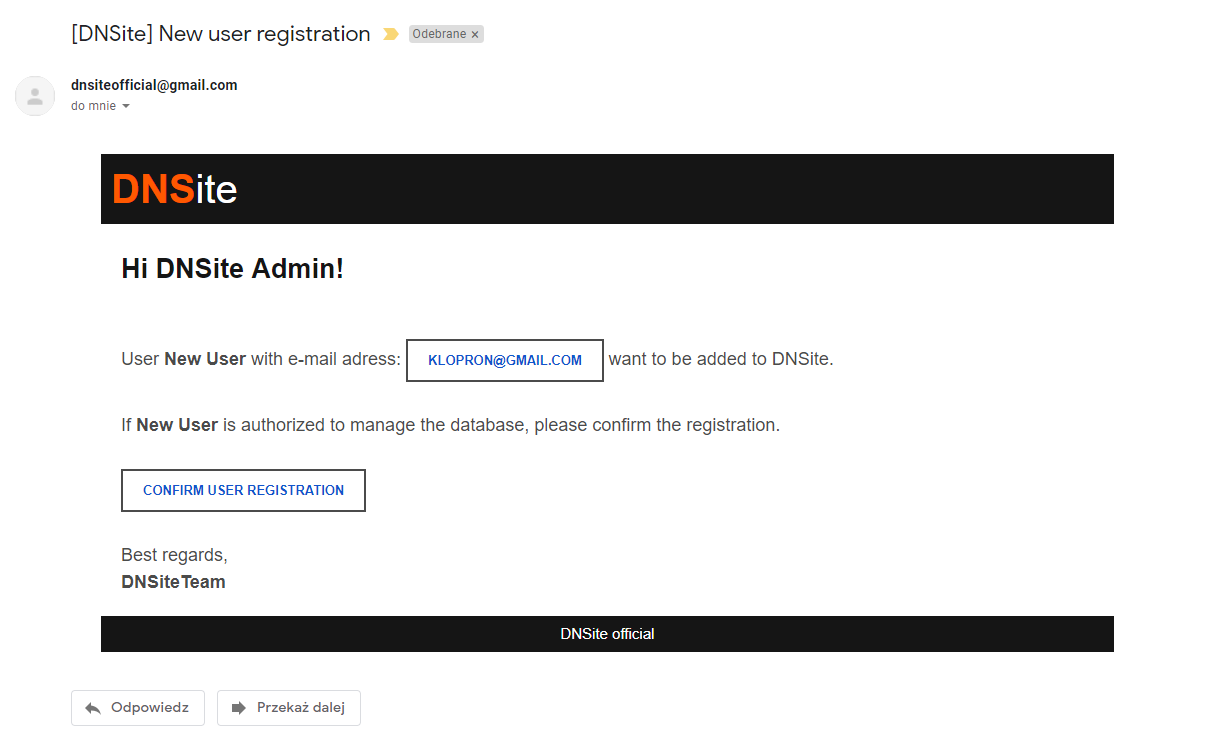
\includegraphics[width=0.8\textwidth]{res/5_mail_potwierdzenie}
\end{figure}

\subsection{Rodzaje kont w aplikacji DNSite}
Aplikacja wyróżnia dwa rodzaje kont:
\begin{itemize}
\item konta zatwierdzone - konta mające pełny dostęp do aplikacji - przy ich pomocy można dokonać logowania. Pierwsze utworzone konto posiada taki status automatycznie.
\item konta niezatwierdzone - konta oczekujące na przyznanie dostępu do aplikacji - dostęp może zostać przyznany przez inne, już zatwierdzone konto
\end{itemize}


\subsection{Przypomnienie hasła}
W sytuacji, gdy użytkownik zapomni hasła do aplikacji, możliwe jest wygenerowanie nowego, tymczasowego. Użytkownik z poziomu panelu logowania powinien wybrać opcję \emph{Remind password}. Zostanie przeniesiony do panelu pokazanego poniżej:
\begin{figure}[H]
\centering
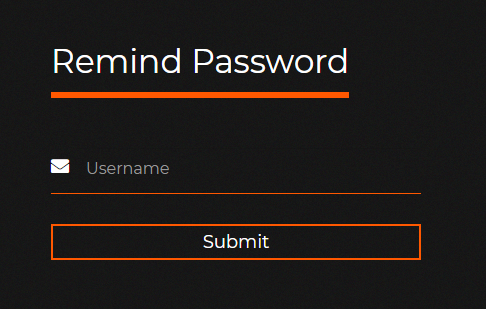
\includegraphics[scale = 1]{res/6_nowe_haslo}
\end{figure}
Po podaniu nazwy użytkownika i wybraniu opcji \emph{Submit}, do użytkownika zostanie wysłana wiadomość e-mail (na adres podany przy rejestracji). Będzie ona zawierać nowe, tymczasowe, wygenerowane losowo hasło, za pomocą którego użytkownik będzie mógł się zalogować do aplikacji. Przykładowa wiadomość została przedstawiona poniżej:
\begin{figure}[H]
\centering
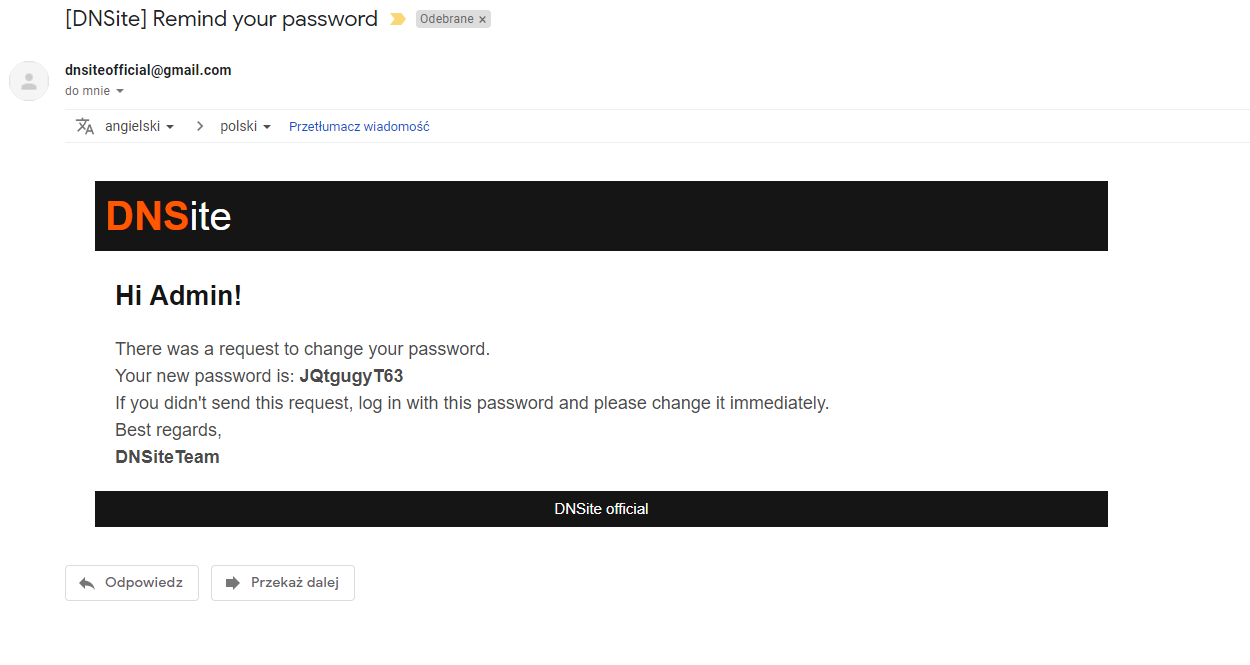
\includegraphics[width=\textwidth]{res/7_mail_haslo}
\end{figure}

\subsection{Strona główna aplikacji}
Po zalogowaniu się do aplikacji użytkownik uzyskuje dostęp do strony głównej:
\begin{figure}[H]
\centering
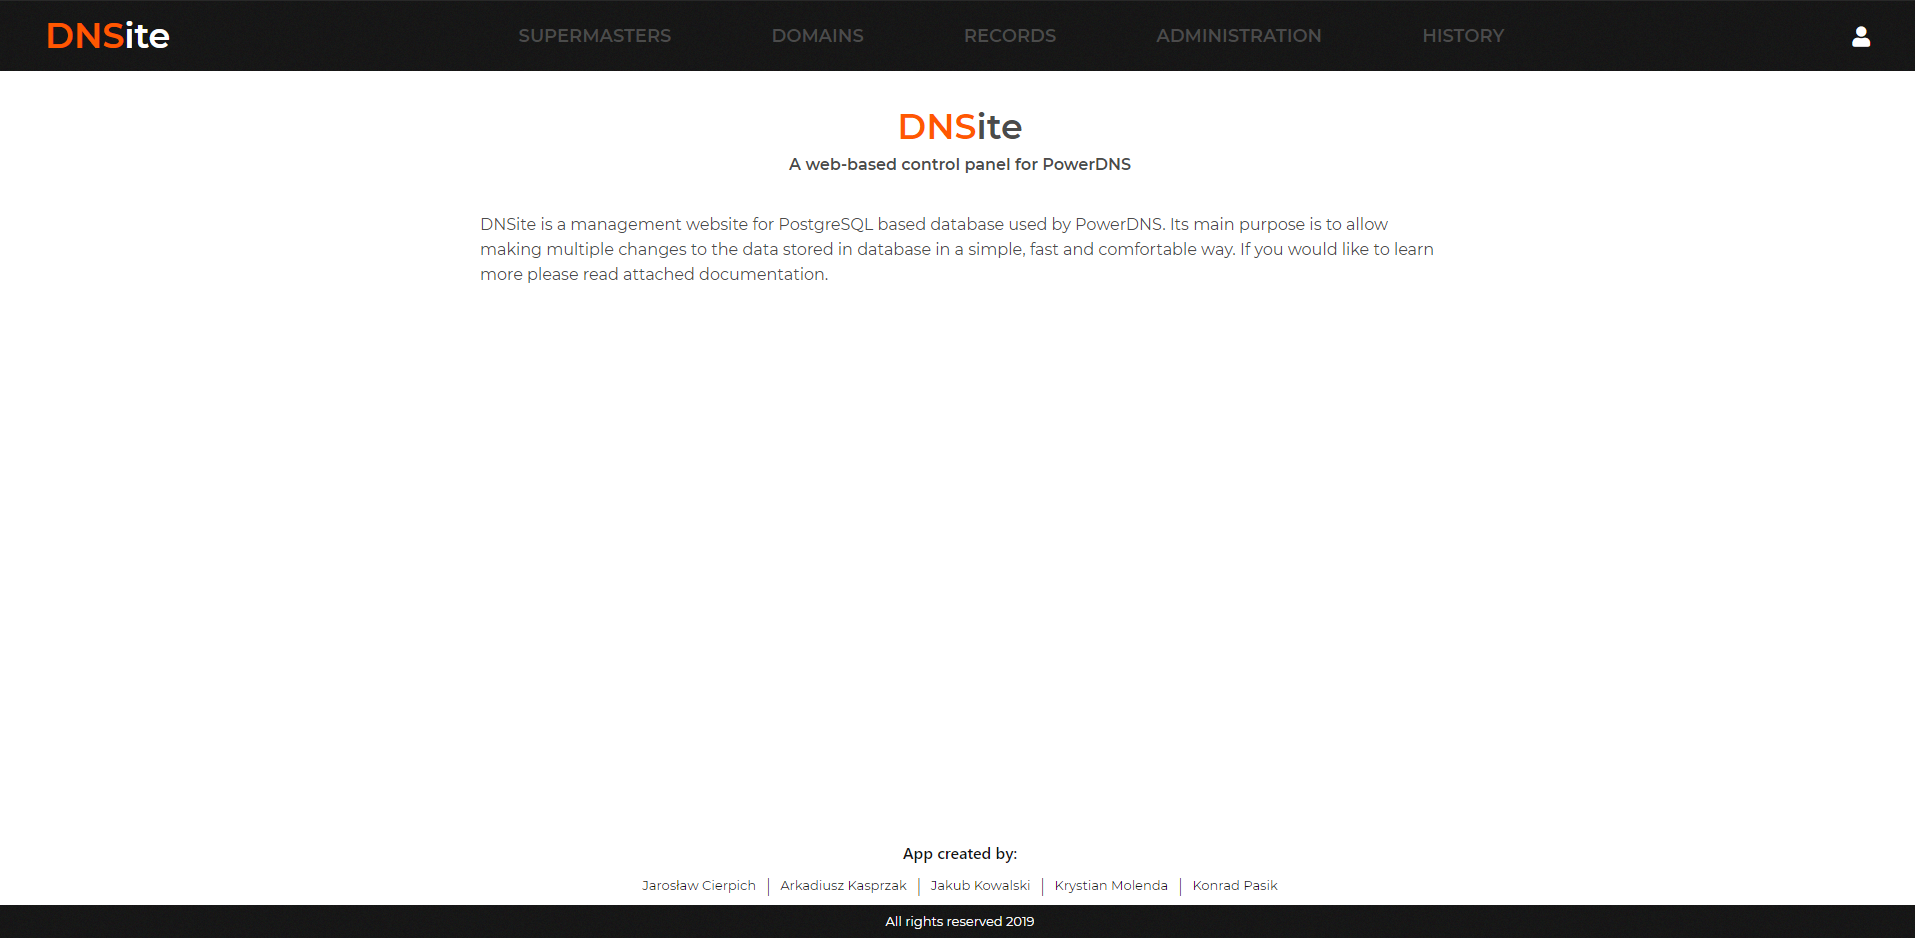
\includegraphics[width=\textwidth]{res/8_strona_glowna}
\end{figure}
W prawym górnym rogu znajduje się \emph{ikona użytkownika} - po jej wciśnięciu pojawia się menu zarządzania kontem:
\begin{figure}[H]
\centering
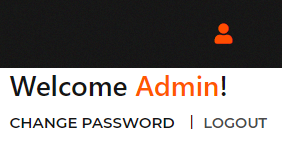
\includegraphics[scale = 1]{res/9_panel_uzytkownika}
\end{figure}
Umożliwia ono \textbf{wylogowanie} się z aplikacji oraz przeniesienie do panelu \textbf{zmiany hasła}. 

Panel nawigacyjny znajdujący się na stronie posiada odnośniki do widoków pozwalających użytkownikowi na przeprowadzenie wszelkich potrzebnych operacji na zasobach aplikacji i serwera DNS. Dostępne opcje:
\begin{itemize}
\item \textbf{Supermasters} - przeprowadzanie modyfikacji tabeli supermasters
\item \textbf{Domains} - przeprowadzanie operacji na domenach DNS
\item \textbf{Records} - przeprowadzanie operacji na rekordach DNS
\item \textbf{Administration} - strona umożliwiająca akceptowanie lub odrzucanie oczekujących na przyjęcie do aplikacji użytkowników
\item \textbf{History} - historia transakcji na bazie danych
\end{itemize}

Dolna część strony zawiera nazwiska autorów aplikacji - kliknięcie nazwiska danego autora przenosi użytkownika do konta w serwisie \textbf{Github}.

\subsection{Operacje na tabelach z danymi}
Rdzeniem funkcjonalności aplikacji \emph{DNSite} jest możliwość przeprowadzania operacji na bazie danych współdzielonej z serwerem \emph{PowerDNS}. W celu przeprowadzenia tychże operacji należy wybrać jedną z następujących opcji:
\begin{itemize}
\item Supermasters
\item Domains
\item Records
\end{itemize}
w panelu nawigacyjnym. W kilku kolejnych podrozdziałach tego poradnika wykorzystany zostanie widok poświęcony rekordom DNS.

\subsubsection{Wstęp do możliwości komponentu tabeli}
Praca na danych oparta jest na tabeli zbudowanej w ten sposób, by ułatwić wykonywanie wielu operacji w krótkim czasie. Komponent tabeli prezentuje się następująco:
\begin{figure}[H]
\centering
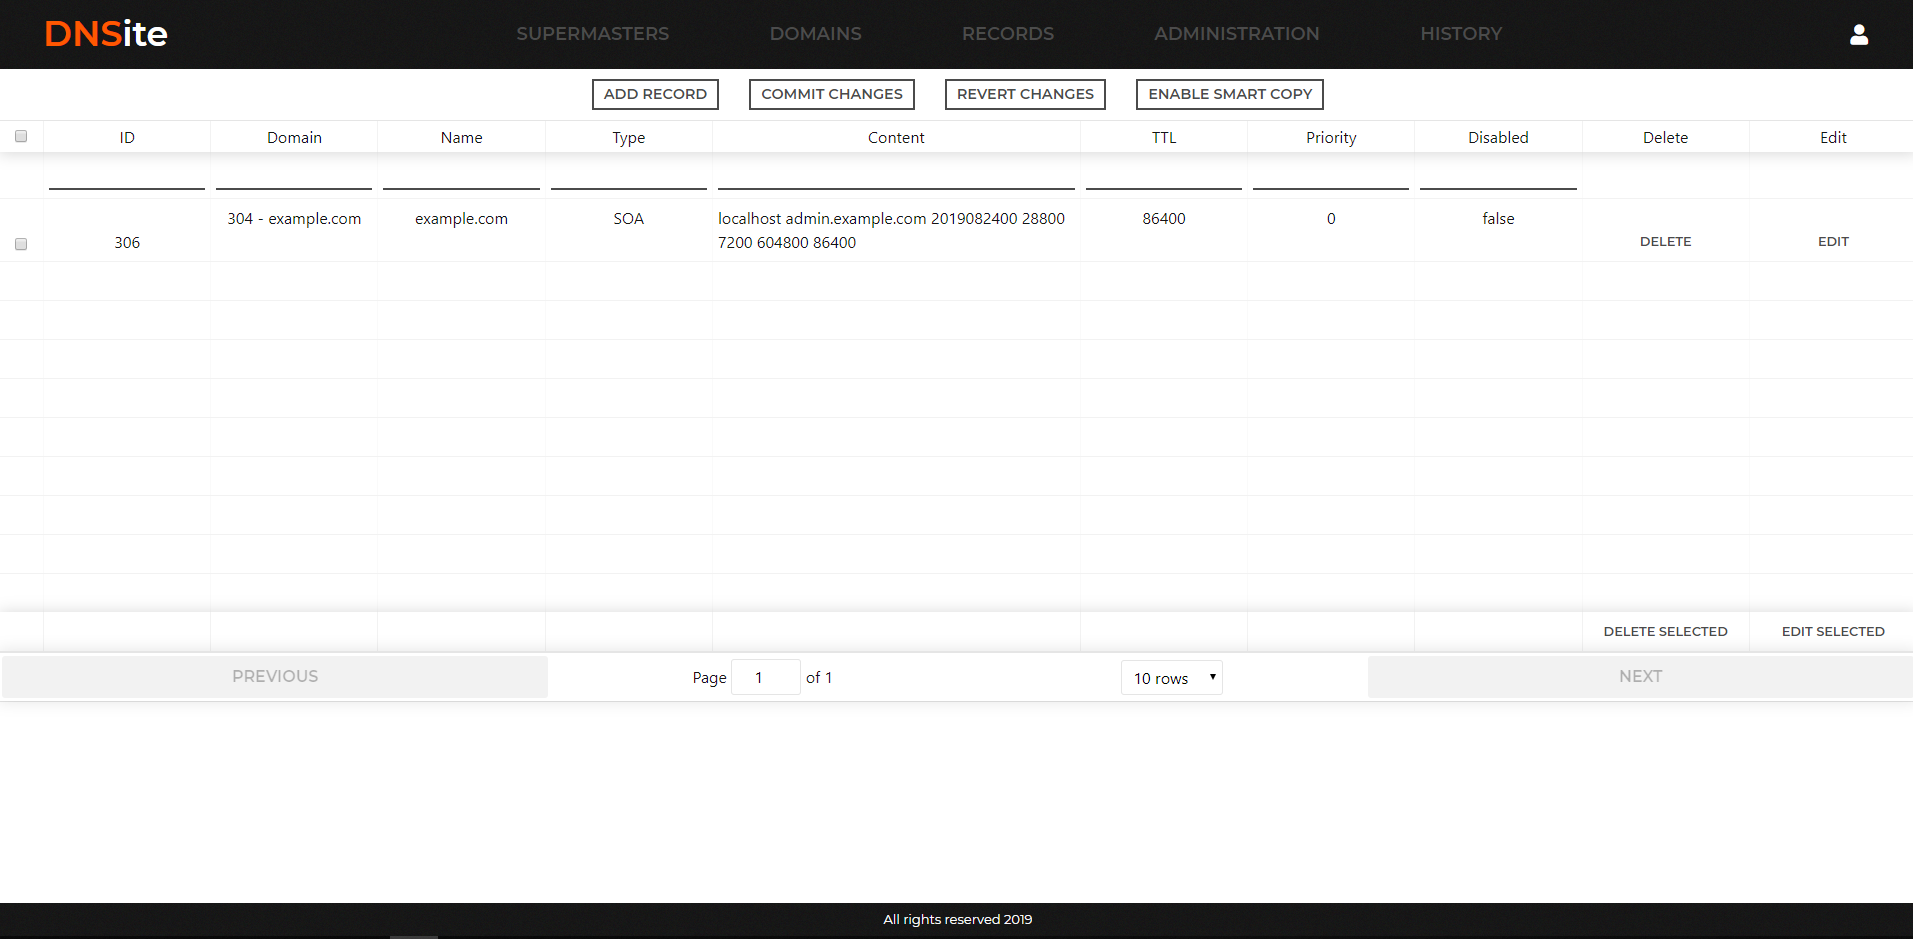
\includegraphics[width=\textwidth]{res/10_tabela}
\end{figure}
W tym przypadku w tabeli znajduje się jeden rekord typu SOA. Wiersz tabeli oprócz danych zawiera:
\begin{itemize}
\item tzw. \emph{checkbox} (po lewej) pozwalający zaznaczyć rekord - służy to do wybierania rekordów, na których mają zostać przeprowadzone operacje działające na wielu rekordach jednocześnie
\item przycisk \emph{Delete} - usuwa rekord z tabeli - rekord jest wtedy dalej widoczny w tabeli - zmienia się przezroczystość wiersza - można go przywrócić za pomocą pojawiającego się wtedy przycisku \emph{Undo Delete}
\item przycisk \emph{Edit} - pozwala włączyć tryb edytowania danego rekordu
\end{itemize}
Komponent tabeli oprócz wyświetlania wierszy pozwala wykonywać wiele innych operacji:
\begin{figure}[H]
\centering
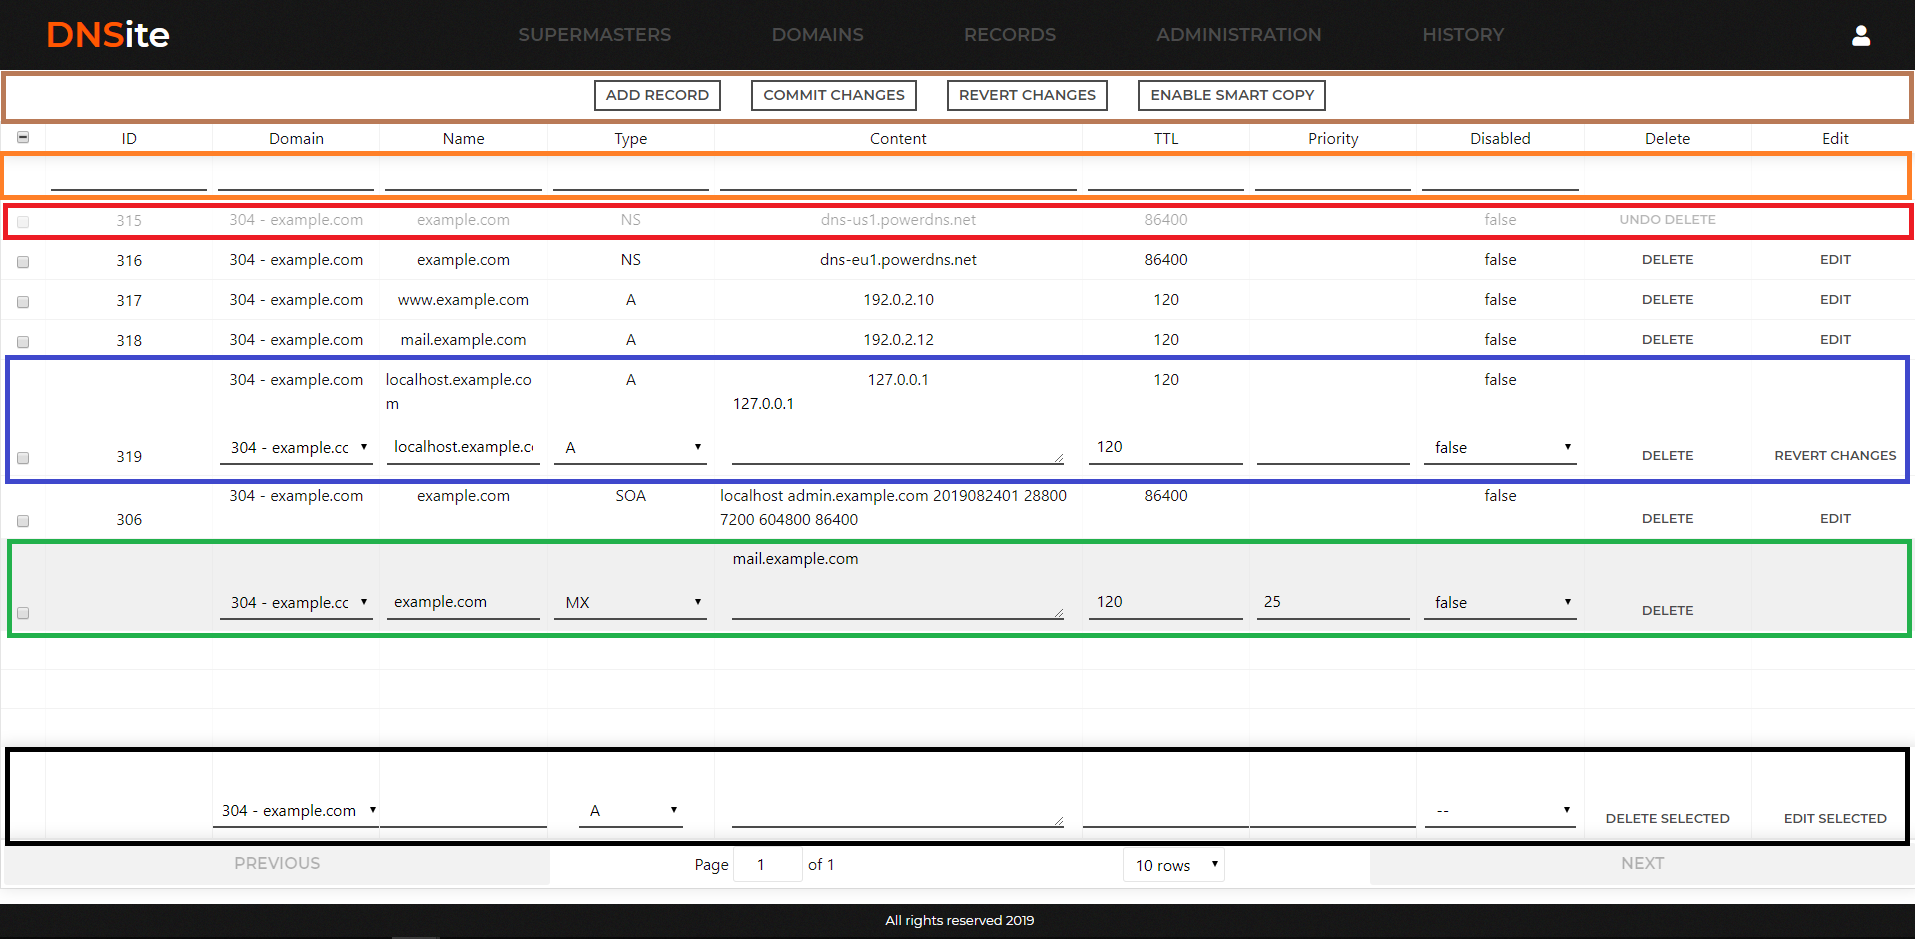
\includegraphics[width=\textwidth]{res/11_tabela_komponenty}
\end{figure}
\begin{itemize}
\item \color{darkbrown} Menu główne tabeli:
\begin{itemize}
\item Dodanie nowego rekordu
\item Zaaplikowanie wszystkich zmian i zaktualizowanie bazy danych
\item Powrót do stanu początkowego - cofnięcie zmian niezaaplikowanych do bazy danych
\item Tryb Smart Copy - opisany w dalszej części poradnika
\end{itemize} \color{black}
\item \color{orange} filtrowanie danych w tabeli \color{black}
\item \color{ao} edytowanie rekordu - wyświetlane są dane aktualnie przechowywane w bazie danych oraz pod nimi pola pozwalające na wprowadzenie nowych danych \color{black}
\item \color{red} usuwanie rekordu - rekord usunięty zostaje oznaczony poprzez zwiększenie jego przezroczystości w tabeli \color{black}
\item \color{forestgreen(web)} nowy wpis w tabeli \color{black}
\item \color{black} wprowadzenie zmian do wszystkich zaznaczonych, aktualne edytowanych rekordów
\end{itemize}


\subsubsection{Zatwierdzenie zmian}
Po wybraniu opcji \emph{Commit changes}, jeśli nie wystąpiły błędy związane z walidacją danych, użytkownikowi zaprezentowana zostaje tabela przedstawiająca wszystkie wprowadzone przez niego zmiany:
\begin{figure}[H]
\centering
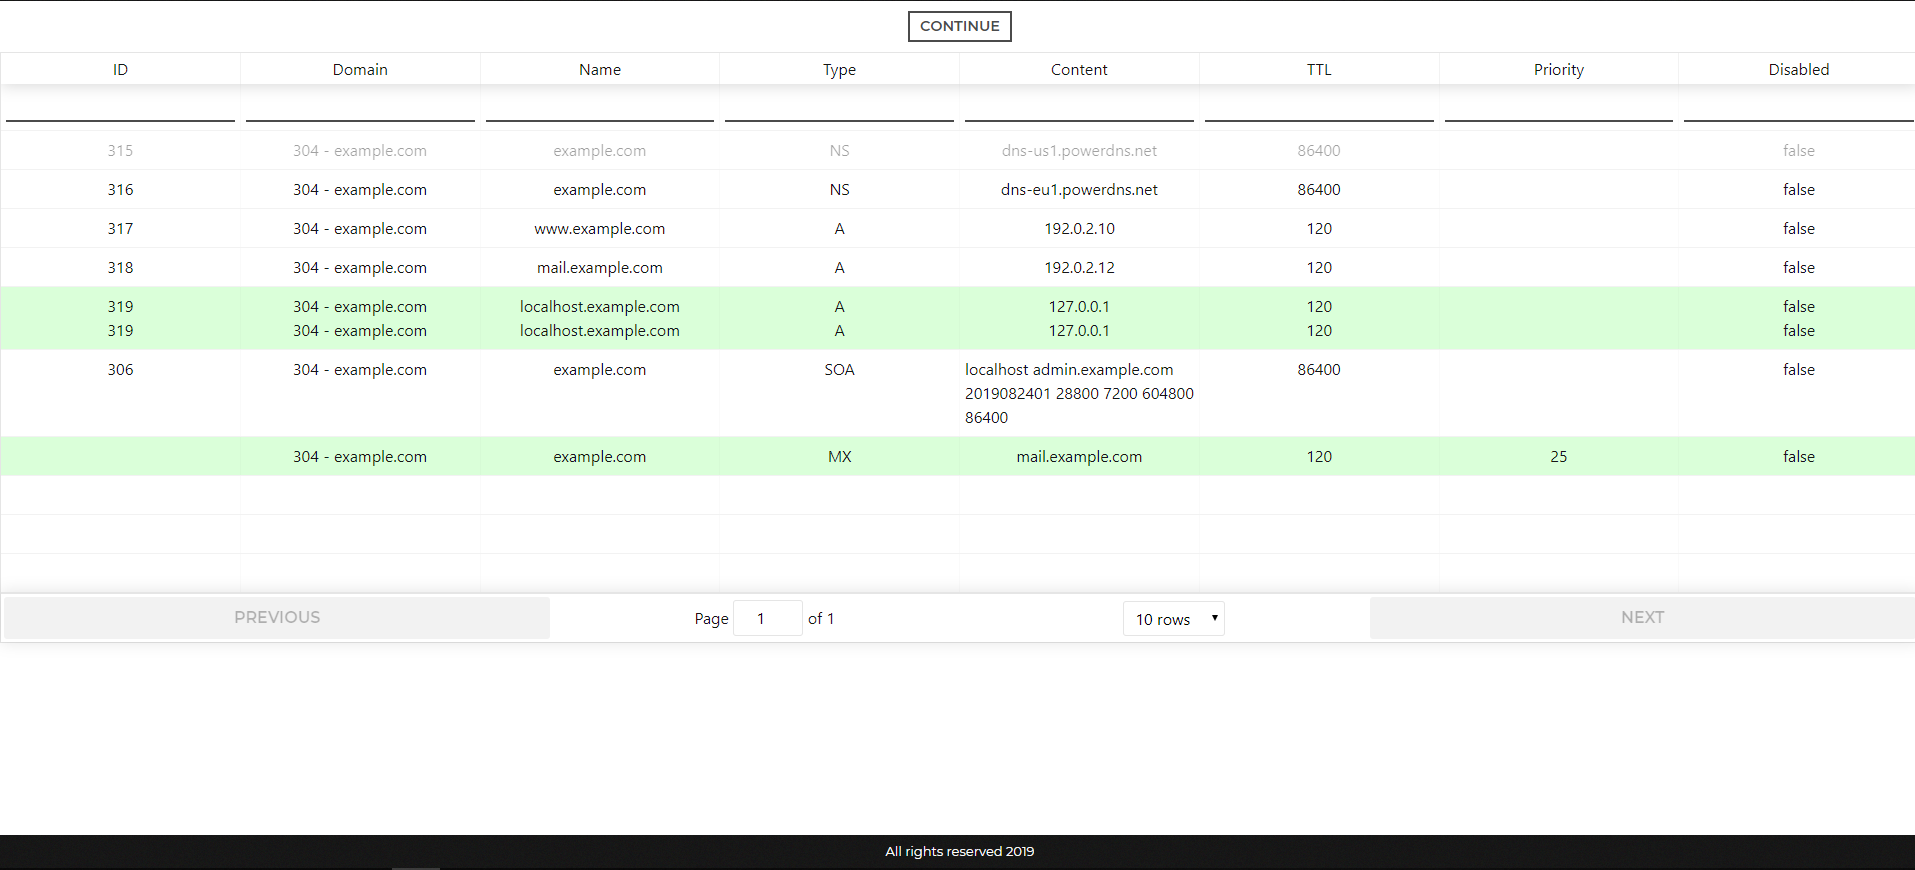
\includegraphics[width=\textwidth]{res/12_tabela_commit}
\end{figure} 
Na zielono zaznaczone zostały rekordy dodane lub zmodyfikowane, rekordy usunięte mają natomiast zwiększoną przezroczystość. Zmian na tym etapie nie można już cofnąć. Aby wrócić do widoku pozwalającego na edycję danych należy wybrać opcję \emph{Continue}.

\subsubsection{Walidacja wprowadzanych danych}
Aplikacja posiada mechanizm walidacji danych wprowadzanych do bazy. W momencie wybrania opcji \emph{Commit changes} sprawdzana jest poprawność danych (np. czy mają one format adresu IP). Jeśli dane zawierają błędy, to nie są wprowadzane do bazy, a użytkownik zostaje o tym poinformowany:
\begin{figure}[H]
\centering
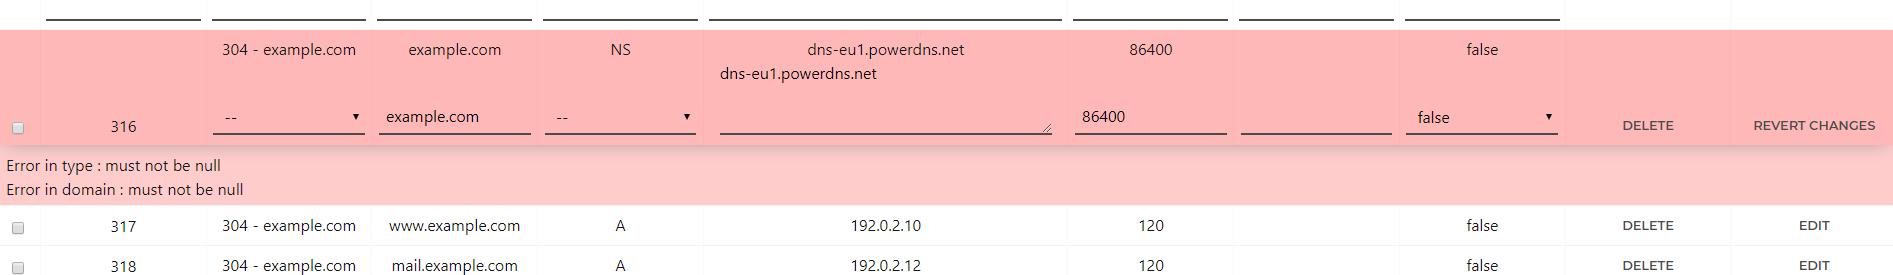
\includegraphics[width=\textwidth]{res/13_tabela_niepoprawny}
\end{figure}
Wiersze zawierające błędy zostają oznaczone kolorem czerwonym. Pod wierszem zostają wypisane znalezione błędy. 

\subsubsection{Zaznaczanie wierszy i komórek tabeli}
Kliknięcie lewym przyciskiem myszy na wiersz tabeli zaznacza go, co zostaje uwidocznione przez zmianę jego koloru:
\begin{figure}[H]
\centering
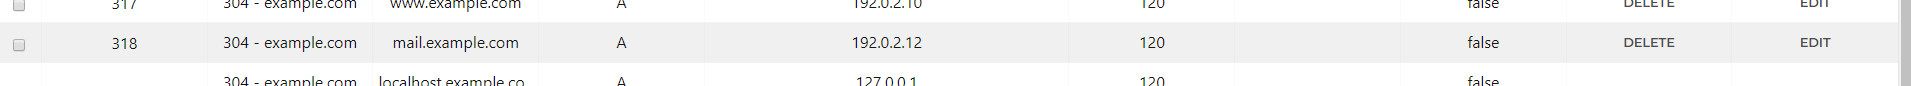
\includegraphics[width=\textwidth]{res/14_tabela_zaznaczenie_wiersz}
\end{figure}
Wykonanie tej samej akcji, ale trzymając przycisk \emph{Ctrl} powoduje zaznaczenie jedynie pojedynczej komórki (przy czym nie każdy rodzaj komórki można zaznaczyć):
\begin{figure}[H]
\centering
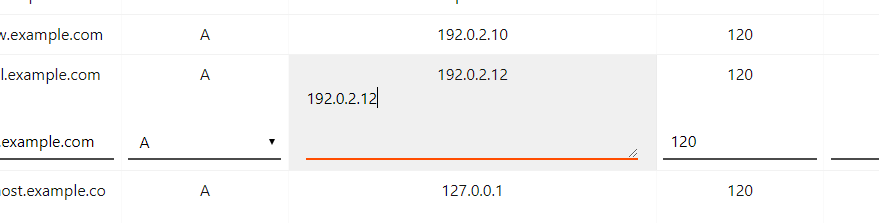
\includegraphics[width=\textwidth]{res/15_tabela_zaznaczenie_pojedyncze}
\end{figure}
Kliknięcie poza obszar tabeli powoduje odznaczenie aktualnie zaznaczonego wiersza/komórki.
Mechanizm zaznaczania jest istotny w połączeniu z opisanym dalej w poradniku mechanizmem Smart Copy. 

\subsubsection{Tryb Smart Copy}
Menu główne tabeli zawiera opcję \emph{Enable Smart Copy} - pozwala ona włączyć mechanizm zmieniający sposób działania kopiowania w tabeli. 

Gdy mechanizm ten jest wyłączony, skróty:
\begin{itemize}
\item \emph{Ctrl+C}
\item \emph{Ctrl+X}
\item \emph{Ctrl+V}
\end{itemize}
spełnią swoje domyślne funkcje. Włączenie trybu \textbf{Smart Copy} zmienia sposób ich działania.

Przy włączonym mechanizmie Smart Copy znaczenie tych skrótów zostaje zmienione:
\begin{itemize}
\item \emph{Ctrl+C} - wykonuje całego zaznaczonego wiersza/komórki, używając wartości znajdujących się w bazie danych - tzn. kopiuje wersję przed modyfikacją
\item \emph{Ctrl+X} - jak wyżej, ale kopiuje zmodyfikowane dane z wiersza
\item \emph{Ctrl+V} - dokonuje wstawienia danych do zaznaczonego wiersza/komórki. Wstawiane są ostatnio skopiowane dane (przy czym nie ma rozróżnienia na kopiowanie za pomocą Ctrl+C i Ctrl+V). Aby skrót zadziałał, wiersz musi być edytowany.
\end{itemize} 

\subsubsection{Modyfikowanie wielu danych jednocześnie}
Stopka tabeli dostarcza kilku opcji modyfikacji wielu danych jednocześnie. Każdej modyfikowalnej kolumnie odpowiada pole w stopce. Aby zmodyfikować kilka wierszy jednocześnie, należy zaznaczyć je za pomocą \emph{checkbox'a} po lewej stronie i wybrać opcję \textbf{Edit selected} - każdy zaznaczony wiersz zostanie przeniesiony w tryb edycji. Następnie za pomocą pól w stopce można wprowadzać dane do wszystkich wierszy, które są jednocześnie zaznaczone i edytowane. Ponadto udostępniona została opcja \textbf{Delete selected} - pozwala ona usunąć jednocześnie wiele wierszy w tabeli. 


\subsection{Dodatkowe opcje operacji na domenach DNS}
Tabela domen udostępnia dodatkowe funkcjonalności niedostępne dla innych widoków. W tej tabeli numer ID domeny jest \textbf{odnośnikiem} do osobnego widoku poświęconego danej domenie:
\begin{figure}[H]
\centering
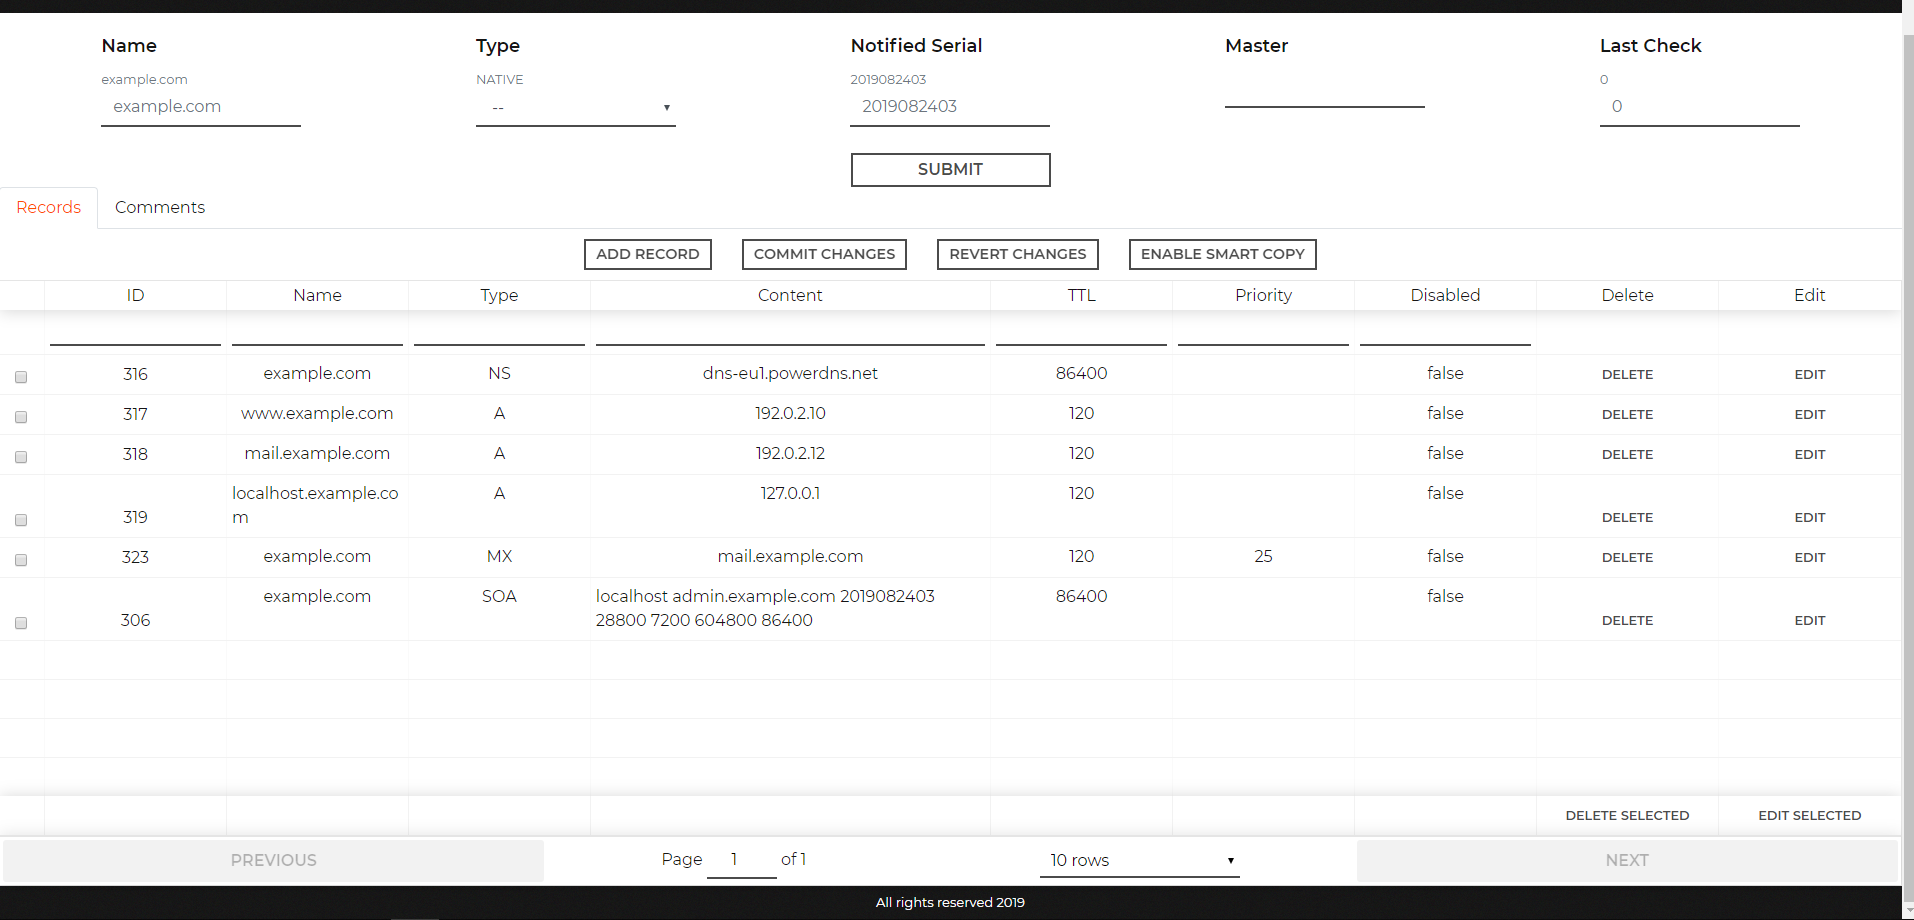
\includegraphics[width=\textwidth]{res/16_widok_domeny}
\end{figure}
Z poziomu tego widoku użytkownik może edytować dane domeny - za pomocą dedykowanego formularza, przeglądać i edytować rekordy powiązane z tą domeną oraz dodawać \textbf{komentarze} - służy do tego tabela w zakładce \emph{Comments}.


\subsection{Panel administratora}
Wybierając opcję \textbf{Administration} w panelu nawigacyjnym użytkownik zostaje przeniesiony do widoku panelu administracyjnego:
\begin{figure}[H]
\centering
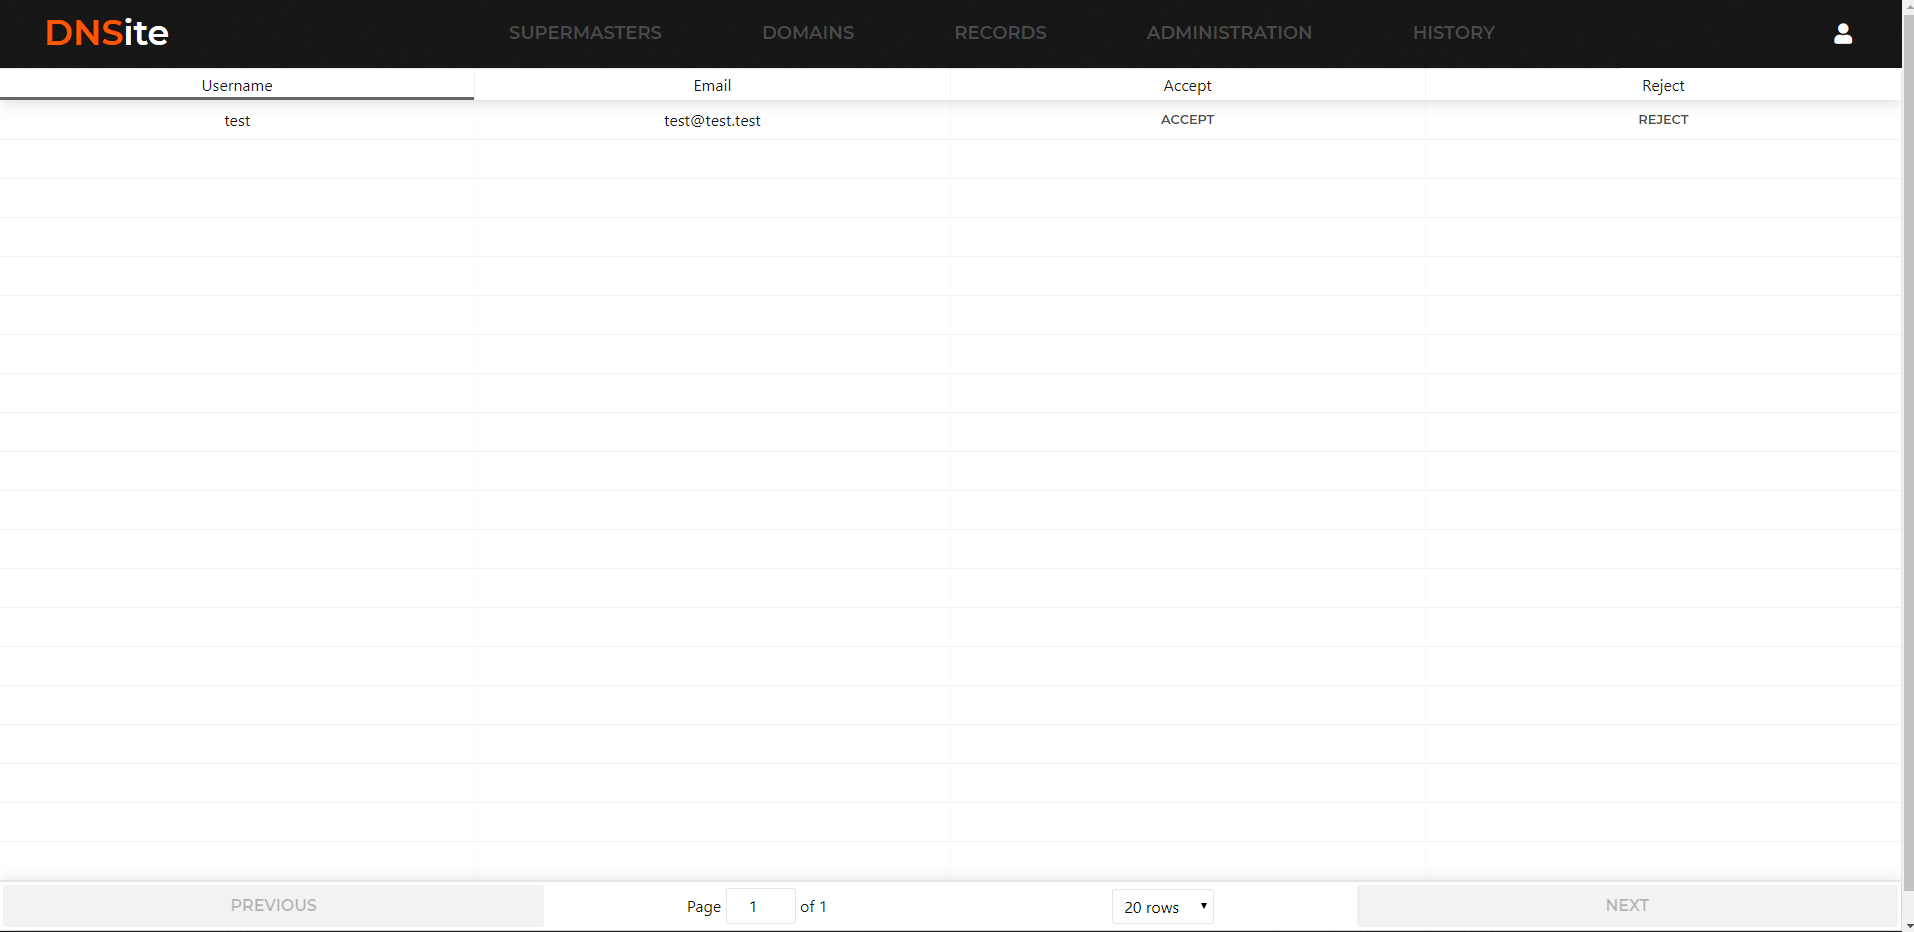
\includegraphics[width=\textwidth]{res/17_panel_administracyjny}
\end{figure}
Z poziomu tego panelu możliwe jest zatwierdzanie lub odrzucanie użytkowników oczekujących na przyznanie dostępu do aplikacji - można tego dokonać kolejno za pomocą przycisków \emph{Accept} oraz \emph{Reject}.

\subsection{Panel historii}
Wybierając opcję \textbf{History} w panelu nawigacyjnym użytkownik zostaje przeniesiony do tabeli zawierającej historię transakcji przeprowadzanych na bazie danych:
\begin{figure}[H]
\centering
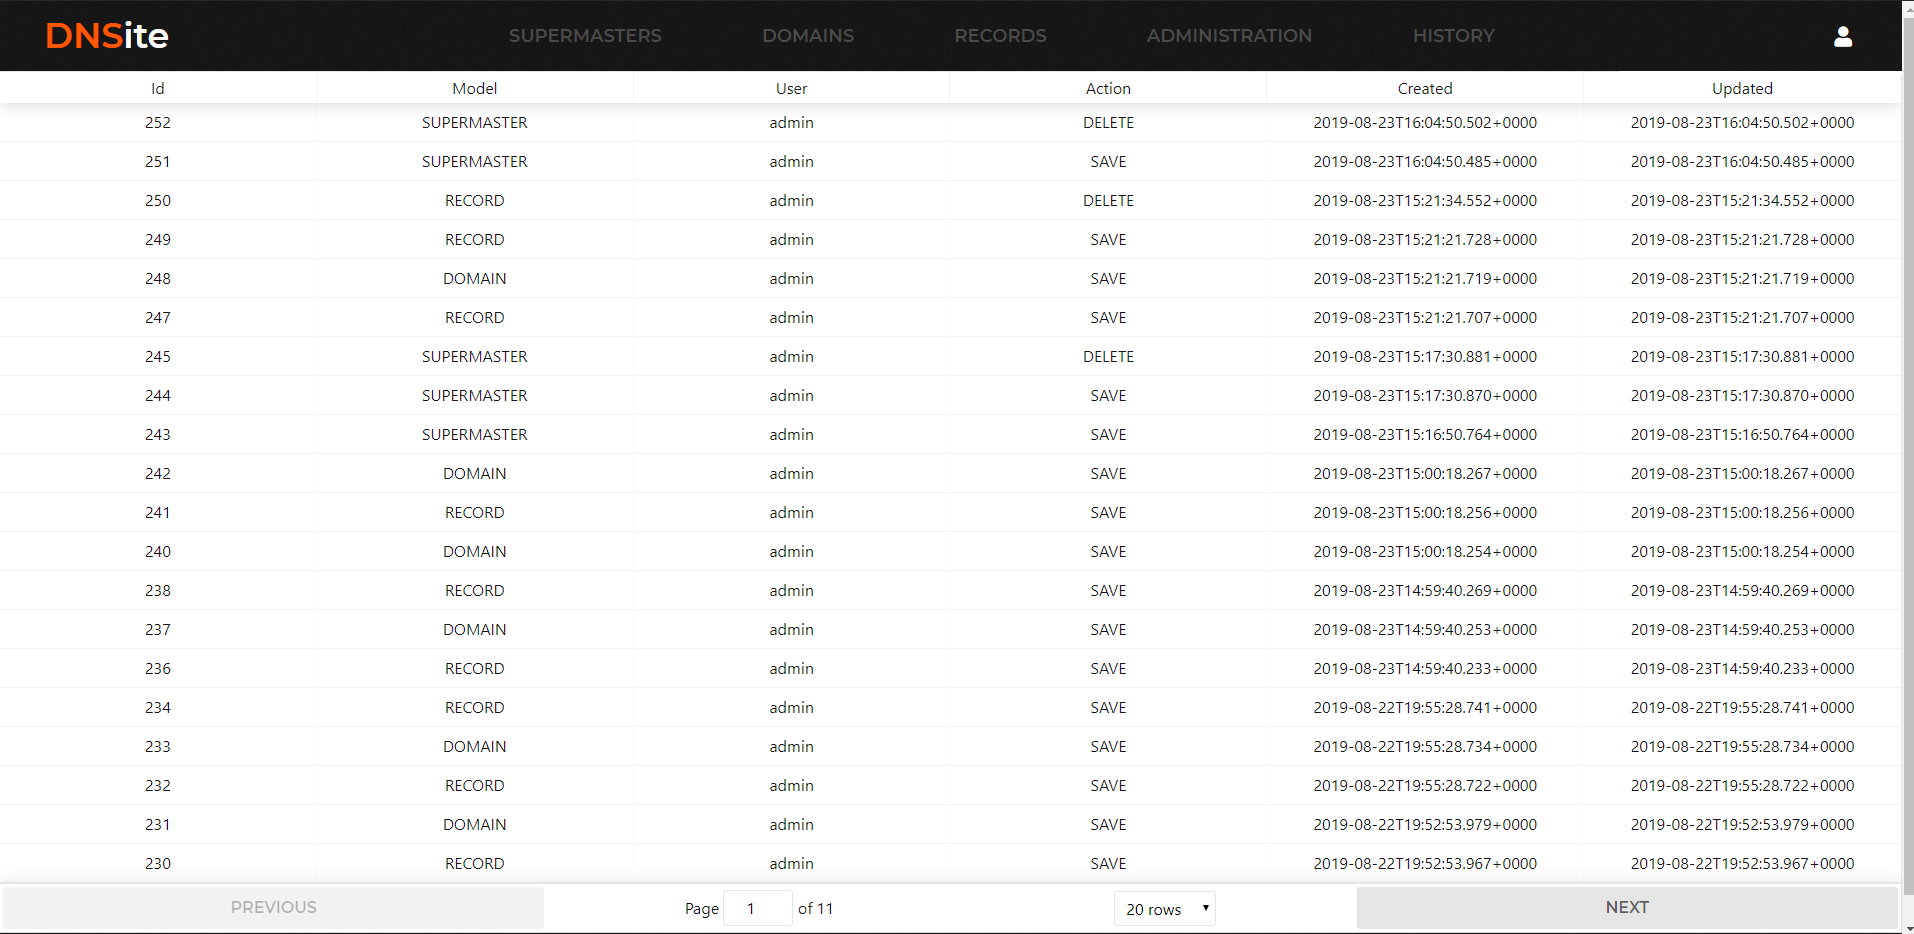
\includegraphics[width=\textwidth]{res/18_historia}
\end{figure}
Z tego poziomu użytkownik może przeglądać jakie zmiany w bazie zostały wprowadzone oraz kto je wprowadził. Kolumna \emph{Model} pokazuje, na jakim zasobie w bazie danych zmiana została przeprowadzona. 


\subsection{Panel zmiany hasła}
Aplikacja udostępnia specjalny panel do zmiany hasła. Opcja ta dostępna jest z poziomu panelu użytkownika (\textbf{Change password}).
\begin{figure}[H]
\centering
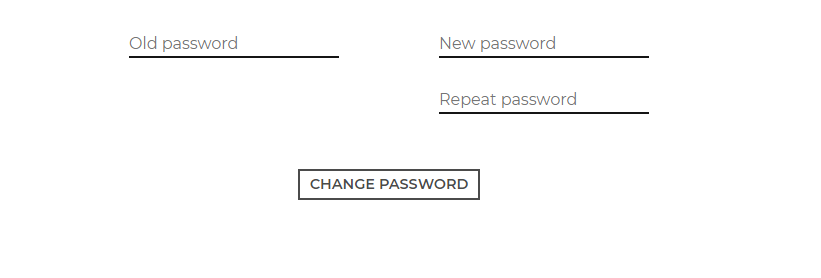
\includegraphics[width=\textwidth]{res/19_zmiana_hasla}
\end{figure}
Użytkownik proszony jest o podanie swojego starego hasła oraz o dwukrotne powtórzenie nowego.


\end{document}